\section{Полная синхронизация}
\begin{enumerate}[\thesection .1]
	\item Находясь в меню <<Синхронизация>> (рис.\ref{pic:pic5}). Необходимо нажать кнопку дополнительного меню внизу экрана планшета. На разных планшетных ПК эта кнопка может выглядеть по разному. В общем случае она обозначается как три точки или три линии.
	После нажатия появится возможность выбрать тип синхронизации
	(рис.\ref{pic:pic9_1})
	\begin{figure}[!h]
		\begin{floatrow}
			\ffigbox{\caption{Выбор типа синхронизации}\label{pic:pic9_1}}%
			{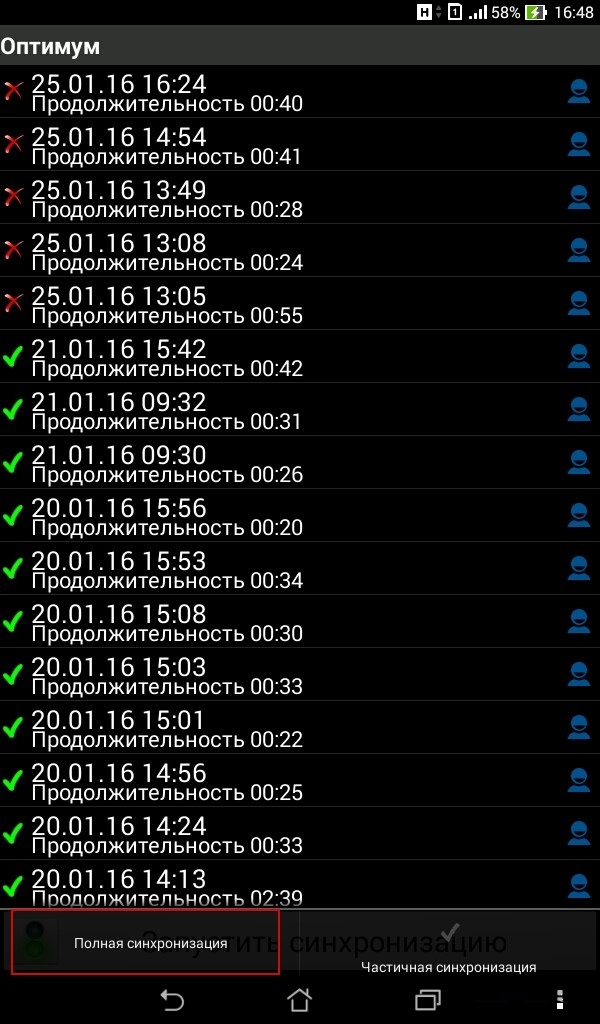
\includegraphics[width=0.8\linewidth]{scr9_1.jpg}}
		\end{floatrow}
	\end{figure}
	Нужно отметить тип <<Полная синхронизация>>, а затем запустить синхронизацию
\end{enumerate}
